% Opciones empleadas:
%
%	a4paper -> indica el tama�o del papel, en este caso A4.
%	11pt -> tama�o de la fuente 11 puntos.
%	oneside -> s�lo escribimos en una cara del folio.
% 
% Otras opciones interesantes:
%
%	twoside -> escribimos a doble cara.
%	openbib -> para que las referencias bibliogr�ficas tengan un salto de l�nea entre cada campo de la referencia.
%
\documentclass[a4paper,11pt,twoside]{book}

% codificaci�n latin1 y s�mbolos del idioma espa�ol (�, acentos, ...)
\usepackage[english]{babel}
\usepackage[latin1]{inputenc}

% puede que queramos usar el s�mbolo del euro.
\usepackage{eurosym}

% El paquete fancybox nos permite crear cajas de diferentes estilos con facilidad.
% http://www.ctan.org/get/macros/latex/contrib/fancybox/fancybox.pdf
% http://www.mackichan.com/index.html?techtalk/487.htm~mainFrame
\usepackage{fancybox}
\usepackage{multicol}
\usepackage{amsmath}

% Para incluir subfiguras.
\usepackage{subfigure}

% Para incluir gr�ficos en JPG => compilar con pdflatex.
% \usepackage[pdftex]{graphicx}
\usepackage[pdftex]{graphicx}   % --> LaTex =>PDF con epstodf
\usepackage{epstopdf}

% Para incluir gr�ficos EPS => compilar con latex.
%\usepackage[dvips]{graphicx}

% Para escribir en color...
%
% ... cuando compilamos con el comando ``latex''
%\usepackage[dvips,usenames]{color}
% ... uando compilamos con el comando ``pdflatex''
\usepackage[pdftex,usenames,dvipsnames]{color}

% Espaciado y ajuste de m�rgenes
\usepackage{setspace}
\onehalfspacing
% \doublespacing
\setlength{\textwidth}{15cm}
\setlength{\textheight}{22cm}
\setlength{\oddsidemargin}{1cm}
\setlength{\evensidemargin}{1cm}
%\usepackage[hmargin={4cm,2.5cm},tmargin=4cm,bmargin=4cm]{geometry}
%Code snippets.
\usepackage{listings}
%Landscape figures.
\usepackage{lscape}

% Paquete fancyhdr -> Para modificar la cabecera y pie de p�ginas.
% http://tug.ctan.org/tex-archive/macros/latex/contrib/fancyhdr/
\usepackage{fancyhdr}
\pagestyle{fancy}
\fancyhf{}
%\fancyhf[HR]{\thepage}
%\fancyhf[HL]{\nouppercase\rightmark}
\fancyhead[LO]{\leftmark}
\fancyhead[RE]{\rightmark}
\fancyhead[RO,LE]{\thepage}
\renewcommand{\chaptermark}[1]{\markboth{\textbf{\thechapter. #1}}{}}
\renewcommand{\sectionmark}[1]{\markright{\textbf{\thesection. #1}}}
\renewcommand{\headrulewidth}{0.6pt}
\setlength{\headheight}{2.5\headheight}

% Package booktabs -> Para mejorar el aspecto de las tablas o cuadros.
% http://www.ctan.org/tex-archive/macros/latex/contrib/booktabs/
\usepackage{booktabs}

% Package rotating -> Para poder girar las tablas y dibujarlas a lo largo
% del folio en vez de a lo ancho.
\usepackage{rotating}

% Packages multicol y multirow, para manejar tablas de filas y columnas m�ltiples.
\usepackage{multicol}
\usepackage{multirow}
%To center the captions.
\usepackage[center]{caption}

%Links in biblio.
\usepackage{url}

\usepackage[pagebackref=true, hypertexnames=true, plainpages=false]{hyperref}

%Bold colors
\usepackage{color,soul}

%Math caligraphy
\DeclareMathAlphabet{\mathpzc}{OT1}{pzc}{m}{it}

%\usepackage[T1]{fontenc}

% Personalizamos la separaci�n entre p�rrafos...
\parskip=6pt

% Personalizamos el identado en la primera l�nea del nuevo p�rrafo...
\parindent=0pt

% Establecemos el n�mero m�ximo de niveles de profundidad en las secciones.
\setcounter{secnumdepth}{3}

%C++ symbol
\def\CC{{C\nolinebreak[4]\hspace{-.05em}\raisebox{.4ex}{\tiny\bf ++}}}

% T�tulo
\title{Design and implementation of a HPC solution for stereo matching}
% Autor
\author{Luis Omar Alvarez Mures}
% Fecha
\date{\today}


\begin{document}

	% \maketitle sirve para generar autom�tica una portada predefinida, pero para un proyecto fin de carrera
	%	de FIC no sirvir�a porque no cumple las normas de presentaci�n. Podemos hacer dos cosas:
	% 1. Usarla e ignorar las normas (y asumir las consecuencias que pueda tener)
	% 2. Hacernos una portada en LaTeX que cumpla las normas (menos arriesgado)
	%
	
	%Modify list bullets so it does not use dash for second level
	\renewcommand{\labelitemi}{$\bullet$}
	\renewcommand{\labelitemii}{$\circ$}
	
	%Change page numbering so backref works
	\pagenumbering{roman}	
	
        %
% Portada.
%

% Nota: Ser�a m�s c�modo emplear el comando \maketitle que genera una portada de forma autom�tica, pero 
% no incluye toda la informaci�n que es necesario incluir en la memoria de un proyecto de fin de carrera
% de la Facultad de Inform�tica de A Coru�a.
%

\begin{titlepage}

  \begin{center}
    
\includegraphics[width=7cm]{figures/anagramaUDC.pdf}\\[0.75cm]
    {\textsc{Faculty of Computer Science}} \\
    {\large \textsc{Departament of Electronics and Systems}} \\[1cm]
    {\Large \textsc{Final Year Project}} \\[0.25cm]
    {\Large \textsc{Master in High Performance Computing}} \\[2cm]
    {\LARGE \textsl{\textbf{Design and implementation of a HPC solution for stereo matching}}} 
    \vfill
    \begin{flushright}
      \begin{tabular}{ll}
        \textbf{Student:}    & Luis Omar �lvarez Mures\\
        \textbf{Advisors:} & Emilio J. Padr�n Gonz�lez\\
        & Juan Ram�n Rabu�al Dopico\\
        & \\
        \multicolumn{2}{r}{\small \emph{A Coru�a, \today{}.}} \\
      \end{tabular}
    \end{flushright}
  \end{center}

\end{titlepage}

        \thispagestyle{empty}
        \cleardoublepage
        %\newpage
	%\thispagestyle{empty}
	%\mbox{}

	% FRONTMATTER: TOC, LOF, LOT y descripci�n/organizaci�n de la memoria.
        \frontmatter
	
	% Los proyectos de fin de carrera de FIC han de ir acompa�ados de una serie de documentos adicionales, algunos
	% 	de ellos obligatorios (certificado, resumen, lista de palabras clave) y otros opcionales (dedicatoria
	%	y agradecimientos).
	%
	
        \thispagestyle{empty}     % No number page, headings...
	\thispagestyle{empty}
\section*{Informaci�n xeral}
\vfill
\begin{center}
  \begin{tabular}{p{4.5cm}p{9cm}}
    \textbf{\emph{T�tulo do proxecto:}} & \textbf{``Dese�o e implementaci�n dunha soluci�n HPC para Stereo Matching''} \\[0.5cm]
    \emph{Clase de proxecto:} & Proxecto de desenvolvemento en investigaci�n \\[0.5cm]
    \emph{Nome do estudante:} & Luis Omar �lvarez Mures \\[0.5cm]
    \emph{Nome dos directores:} & Emilio Jos� Padr�n Gonz�lez \\
    & Juan Ram�n Rabu�al Dopico \\[0.5cm]
    \emph{Membros do tribunal:} & \\[0.5cm]
    & \\
    & \\
    & \\
    & \\
    & \\
    & \\
    & \\
    & \\
    & \\
    & \\
    \emph{Data de lectura:} & \\[0.5cm]
    \emph{Cualificaci�n:} & \\
  \end{tabular}
\end{center}
\vfill

	
	\thispagestyle{empty}
        \cleardoublepage
	
	\thispagestyle{empty}     % No number page, headings...
	%
% Dedicatoria
%
\section*{}

\begin{flushright}
	{\it Dedicated to Rebeca and my parents.}
\end{flushright}

        
        \thispagestyle{empty}
        \cleardoublepage
        
        %\newpage
	%\thispagestyle{empty}
	%\mbox{}
	
	\thispagestyle{empty}
        %
% Agradecimientos
%

\section*{Acknowledgements\footnote{In alphabetical order}}

My sincerest thank you for the help provided:

To Mr. Emilio Jos� Padr�n Gonz�lez.

To Mr. Juan Ram�n Rabu�al Dopico.




        
        \thispagestyle{empty}
        \cleardoublepage
        %\newpage
	%\thispagestyle{empty}
	%\mbox{}
	
	\thispagestyle{empty}
        %
% Resumen del proyecto de fin de carrera
%

\section*{Resumo:}

O obxectivo deste proxecto � o dese�o e implementaci�n dunha
ferramenta multiplataforma para a visualizaci�n de nubes de puntos que
permita a xesti�n e manipulaci�n de grandes volumes de datos. Este
tipo de \emph{datasets} poden ser obtidos a partir dun esc�ner LIDAR
ou de alternativas de baixo custo como KINECT.

Este tipo de sistemas capturan un gran volume de informaci�n, xerando
nubes de puntos de gran tama�o con miles de mill�ns de informaci�n
xeom�trica, color, normais, reflectividade, etc. A consecuencia � un
conxunto de informaci�n dif�cil de manexar de xeito interactivo, ao
non caber completo na memoria RAM dun ordenador e requerir o traballo
desde memoria secundaria (cl�sicamente un disco duro). Isto complica
a creaci�n de aplicaci�ns en tempo real para a xesti�n e manexo deste
conxunto masivo de datos.

A ferramenta software desenvolvida neste proxecto ofr�celle ao usuario
final todas as funcionalidades necesarias para o traballo con este
tipo de datos, desde un completo visualizador 3D para render de
puntos, que incl�e caracter�sticas de visualizaci�n avanzada de
OpenGL, soporte para o traballo con varias nubes de puntos
simultaneamente, m�ltiples c�maras diferentes coas que traballar,
caracter�sticas multiresoluci�n, posibilidade de aplicar
transformaci�ns e distintos tipos de pre-proceso sobre os datos, medir
distancias, detecci�n de obxectos na nube de puntos, exportaci�n a CAD
dos obxectos seleccionados, etc

Para a implementaci�n de todas esas funcionalidades partiuse da
biblioteca software PCM, a�nda en desenvolvemento e que xurde tam�n
na Unidersidade da Coru�a. Este biblioteca proporciona unha serie de
ferramentas de baixo nivel para a xesti�n de nubes de puntos masivas
en hardware de uso com�n. Neste proxecto non soamente se fai uso das
caracter�sticas existentes de PCM, sen�n que, ademais da propia
ferramenta de visualizaci�n desenvolvida (bautizada como ToVIEW), tam�n se extendeu
ampliamente a biblioteca PCM para poder ofrecer todas as funcionalidades
necesarias no proxecto, ademais de varias melloras de rendemento na mesma.

No proxecto abordouse ademais o aproveitamento das posibilidades para
o procesamento paralelo presentes no hardware no que se executa PCM,
tanto en canto � CPU como �s capacidades GPGPU da tarxeta gr�fica.

Por �ltimo, o paquete software resultante foi dese�ado para ser
facilmente integrable nos fluxos de traballo habituais nos sectores da
enxe�er�a que m�is habitualmente empregan escaneos 3D en forma de
nubes de puntos, como pode ser, por exemplo, a topograf�a.
Durante a realizaci�n do proxecto traballouse con profesionais da
topograf�a habituados a incorporar o uso da tecnoloc�a LIDAR no seu
traballo, o que facilitou a creaci�n dunha ferramenta �til e vers�til
para o usuario final.
No aspecto da f�cil integraci�n en entornos profesionais tam�n axuda o
feito de tratarse dun desenvolvemento multiplataforma e \emph{open source}.

        
        \thispagestyle{empty}
        \cleardoublepage
	
	\thispagestyle{empty}
        %
% Resumen del proyecto de fin de carrera
%

\section*{Abstract:}

The objective of this project is designing and implementing a multi-platform point-based rendering visualizer that allows the management and interactive manipulation of big 3D point clouds. These clouds can be obtained using a LIDAR scanner or cheaper alternatives like KINECT. 

These systems can nowadays generate data-sets with huge amounts of point data, position, color, normals, reflectivity, etc. As a consequence, these point clouds will not fit on system RAM and will have to reside in an HDD. Due to this fact, real-time rendering of massive point clouds is a complex task.

The resulting software tool developed in this project, will offer the end user the functionality necessary for working with these types of datasets. Including a complete 3D visualizer, with advanced OpenGL point-rendering capabilities, multiple point cloud support, multiple cameras, multi-resolution capabilities, point cloud transformation and preprocessing, distance measurements, object segmentation, CAD exportation of segmented objects, etc. 

To implement all of these features, we will utilize PCM. PCM is a project in development from the University of A Coru�a, that provides a series of low level tools for working with point clouds on commodity hardware. This project will not only extend PCM with the aforementioned functionality and a high level software tool for the end user, but will improve the existing code and some performance aspects of PCM.

Furthermore, the provided tool will take advantage of all the parallel computing capabilities of the target platforms. Using multiple cores on CPUs and GPGPU on the graphics cards. The multi-resolution framework will also help when trying to achieve maximum performance when trying to apply any computation.

In conclusion, the resulting software package should be easily integrated and improve substantially the existing engineering workflows, thanks to the fact that the tool will be multi-platform and open source. Since it was also developed with the advice of some surveyors that are working with laser scanners everyday, there are high hopes of truly having created a versatile and useful tool.





        
        \thispagestyle{empty}
        \cleardoublepage
        
        \thispagestyle{empty}     % No number page, headings...
	%
% Palabras clave
%

\section*{Lista de palabras chave:}

Motor, render, nubes de puntos, k-d tree, multi-resoluci�n, tiempo real, PCM, ToView, open source, multi-plataforma.

\section*{Keywords:}

Engine, render, point clouds, k-d tree, multi-resolution, real-time, PCM, ToView, open source, multi-platform.



	
	\thispagestyle{empty}
        \cleardoublepage
	
        \thispagestyle{empty}     % No number page, headings...
        %
% Software y Hardware
%

\section*{Hardware e software empregado:}

\begin{itemize}
\item Intel Core i7s, NVIDIA GTXs \& GTs.
\item C++, Visual Studio, Git, OpenCV, OpenMP, OpenCL, CUDA, Boost, GCC.
\end{itemize}



        
        \thispagestyle{empty}
        \cleardoublepage
        
       % \thispagestyle{empty}     % No number page, headings...
        
        %\newpage
	%\thispagestyle{empty}
	%\mbox{}

        \tableofcontents
        \listoffigures
        \listoftables
        
        %\newpage
	%\thispagestyle{empty}
	%\mbox{}

	% MAINMATTER: El contenido, cap�tulo a cap�tulo, de la memoria del tfg.
        \mainmatter
	
	\pagenumbering{arabic}	
	
	%
% Frontmatter - Introducci�n. Los miembros del tribunal que juzgan los PFC's tienen muchas m�s memorias que leer, por lo que
%	agradecer�n cualquier detalle que permita facilitarles la vida. En este sentido, realizar una peque�a introducci�n,
%	comentar la organizaci�n y estructura de la memoria y resumir brevemente cada cap�tulo puede ser una buena pr�ctica
%	que permita al lector centrarse f�cilmente en la parte que m�s le interesa.
%

\chapter[Introduction]{
	Introduction
}

Computer Graphics is the discipline that deals with creating, managing, analyzing and visualizing graphics using a computer, and it is closely linked to other disciplines such as Image Processing, Computer Vision or Machine Learning, among others. Advances in computer graphics have had an impact on several media types such as, for example, the movies and video games industry, civil engineering, medicine, etc.

In computer graphics, \emph{rendering} is the process of generating a 2D image to be shown in a display. This process takes usually a virtual scene of 3D objects as input, containing data like geometry, lighting, cameras, etc.
Typically, polygonal modeling has been the approach followed for modeling objects in the scene, approximating their surfaces using polygons. Point-based graphics focuses on points as the fundamental representation of the surfaces instead of polygons (see \figurename~\ref{poly_comp}).

\begin{figure}
	\centering
	\includegraphics[scale=0.6]{figures/pol_comp.pdf}
	\caption[Modeling types comparison]{
		From left to right; mathematical representation of a plane, representation using two polygons (triangles) and a point-based representation.
	}
	\label{poly_comp}
\end{figure}

Nowadays, acquisition technologies such as LIDAR (Laser Imaging
Detection and Ranging) allow us to obtain high-precision
georeferenced 3D scans of the real world in an easy and fast way.
These systems use ultraviolet, visible or near infrared light to image objects. It can target a wide range of materials and even single molecules. A narrow laser beam can map features with very high precision.
The evolution of this kind of technologies is having a tremendous
impact in multiple fields in the engineering, and bringing back the
camp-work to the office has become a standard practice.
This presents clear advantages compared to the classical work-flow in
disciplines like topography, that usually need to come back on the
ground each time a new measurement is required. A couple of images
obtained from a LIDAR scanner are shown in
\figurename~\ref{lidarexamples}.

\begin{figure}
  \centering
  \includegraphics[width=0.475\textwidth]{figures/campillo1.png} \quad
  \includegraphics[width=0.475\textwidth]{figures/parcela.png}
  \caption{Examples of LIDAR scanning.}\label{lidarexamples}
\end{figure}

These scanning devices generate data-sets with an enormous number of
samples, with 3D coordinates and additional data such as color,
reflectivity and so on. These point clouds, as they are usually
named, are formed by hundreds or thousands of points, resulting in
Giga or even tera-bytes of information.
Using point based representations, the polygonal approximation step
can be skipped and the massive amount of captured data is directly
used. However, managing these huge data-sets, either for applying some kind of data
analysis or for visualization, is a computational challenge and an
open and state-of-the-art problem. This project deals with this question.

This chapter introduces the motivation behind the project and the
objectives we try to achieve. It shows the structure of this document
as well.

\section[Motivation and context]{
	Project motivation and context
}

PCM is a software library developed in the University of A Coru�a for the management of huge point datasets obtained by LIDAR in commodity hardware systems. It was started as a MSc Final Project~\cite{Jaspe12} (system structure and basic capabilities) in the Faculty of Computer Science and then continued in a BSc Final Project~\cite{Jaspe13} (improved render and other minor additions).

PCM is based on a multi-resolution structure and includes basic memory hierarchy management, making it possible to transfer the point cloud data between secondary memory (HDD) and video memory in the graphics card. Originally, PCM includes a very basic visualizer, quite simple and limited but that has the potential to become the seed for a more advanced point cloud software tool that will allow the user to access all of these features in real-time.

Although PCM was designed to deal with arbitrary size datasets, it is far from being a mature software and has some problems managing point clouds in the order of billion points. Because of the massive nature of these datasets, achieving real-time manipulation of them is a complex task. It will require the improvement of PCM, with a complete profiling and performance analysis and a careful refactoring. Having a system that is able to manage such a huge amount of data, will let the user take advantage of the full potential of cutting-edge 3D capture devices.
Of course, the library should exploit the full potential of both modern CPUs and GPUs, automatically using parallel processing to reduce the computation time as much as possible.
Furthermore, although PCM sketches a framework for applying data
analysis on the point clouds, this part was barely crafted at
all. Other constraints of the original proposal are also addressed in
this work, such as adding read/write operations to allow the
modification of the datasets, the possibility of working with multiple
point clouds, etc.

In this project, a complete user-oriented software suite for the visualization, management, analysis and manipulation of massive 3D point clouds will be developed from the original PCM proposal. ToView is the name chosen for this software package. It is a multi-platform (GNU/Linux, Windows and MacOS) free software project and makes use of open source software exclusively. For these reasons the user interface is based on the cross-platform application framework QT, that has native implementations and tools for all the aforementioned platforms. The resulting QT application will let the user access all of the functionality including an advanced and complete 3D visualizer.

\section[Objectives]{
	Project objectives
}

The aim of this project is the design and implementation of a point-based multi-platform software tool for the interactive visualization, management, analysis and manipulation of massive 3D point clouds. 

The application will offer the user the necessary tools to work effectively with this type of datasets, including a 3D visualizer with advanced point-rendering techniques using OpenGL, that will allow real time interaction with one or multiple point clouds.

From the interface, the user will be able to:

\begin{itemize}
\item Select different visualization modes for point-based models: multiple cameras, simple and advanced visualization, multi-resolution, etc.
\item Combine different point clouds with tools that enable rotation, translation and scaling of the datasets.
\item Select points in the clouds for working with them.
\item Apply operations to a part of the cloud or the complete dataset. From simple operations, such as distance measurement and calculation, to plane or other geometric primitives detection.
\item Export the work done to a standard CAD format, so the tool can be integrated in other work-flows.
\item Call the pre- and post-processing tools included in the suite: multi-resolution structure computation, filters, etc.
\end{itemize}

The developed tool will take advantage of the parallel computing possibilities of the platforms. Both using the GPGPU capabilities of the graphics card with OpenCL and the multiple cores of the CPU. 

PCM will be used as the foundation for this work. PCM is a project in development that offers several low level tools for working with point clouds of arbitrary size in commodity hardware, from which a multi-resolution structure with different levels of cache is highlighted. This final degree project will not only extend PCM with the mentioned features, offering a high level software suite for the final user, but will also improve the existing source code, paying special attention to performance aspects.

A series of benchmarks will also be implemented that will allow us to obtain automatically and autonomously performance information about PCM and the visualization tool, with graphs and reports. This tool will make finding bottlenecks and performance issues easier.

\section[Structure]{
Document structure
}

The rest of the document is organized following this structure:

\paragraph*{Chapter 2.}
Planning and methodology

After this introduction, we start by describing the planning and
development methodology used in the project. We chose an agile
software development approach.

\paragraph*{Chapter 3.}
Computer Graphics basics

This chapter briefs the very basic concepts about computer graphics needed to understand the rest of the document: How a virtual camera works and the different types of cameras, what 3D transformations are and how a point is represented in 3D.
 
\paragraph*{Chapter 4.}
Structure of a real-time visualizer for point-based datasets

This chapter describes the structure of the visualizer we propose in this work and presents the class diagram of the software package. Both ToView (the visualization tool) and PCM (the multi-resolution library behind the GUI) are included.

\paragraph*{Chapter 5.}
Point Cloud Manager

This chapter focussed in describing PCM ant detailing all the work
invested in the improvement of the original PCM library and tools:
code refactoring, bug fixes and new functionalities. It includes the
experimental results of the tests included in the benchmarks we have
designed to measure the library performance.

\paragraph*{Chapter 6.}
ToView

This chapter depicts the visualizer designed and implemented from
scratch in this project to manage and visualize massive point
clouds. All the included functionalities are described and
experimental results are also included.

\paragraph*{Chapter 7.}
Advanced GPU point rendering

This chapter is devoted to the most advanced visualization methods
included in ToView, a bunch of some of the most state-of-the-art
point-rendering techniques, and how they are implemented with OpenGL
in the GPU using GLSL (OpenGL Shading Language).

\paragraph*{Chapter 8.}
Object detection: RANSAC

This chapter deals with the detection of different shapes and volumes
in ToView, describing the different approaches that were studied to implement
this functionality in the project. Specifically, an extensive
explanation of the RANSAC algorithms used in this project is provided.

\paragraph*{Chapter 9.}
Preprocessing and filtering

Both PCM and ToView need several pre-processing tasks to take advantage
of some of the most advances features. All this pre-processing and the
different filtering techniques applied to the datasets are explored in
this chapter.

\paragraph*{Chapter 10.}
Conclusions and future lines of work

Finally, this chapter presents the main conclusions obtained with this
project and outlines possible extensions to both PCM and ToView.

	%
% T�TULO DEL CAP�TULO
%
\chapter{Technological Foundations
	\label{chapter_2}
}

In this chapter, some Computer Vision concepts are introduced. Paying special attention to our case study that is stereo correspondence. We first introduce what is computer vision and delve into our case study, second we explain the chosen Stereo Matching algorithm and third describe what GPGPU is and its applications in our area of interest. Only a brief description of these concepts is presented, to get more familiarized with Computer Vision the books \cite{computervision} and \cite{computervisionmodern} are recommended. For stereo correspondence techniques, the book chapter \cite{correspondence} is an essential source.

\begin{figure}[h]
	\centering
	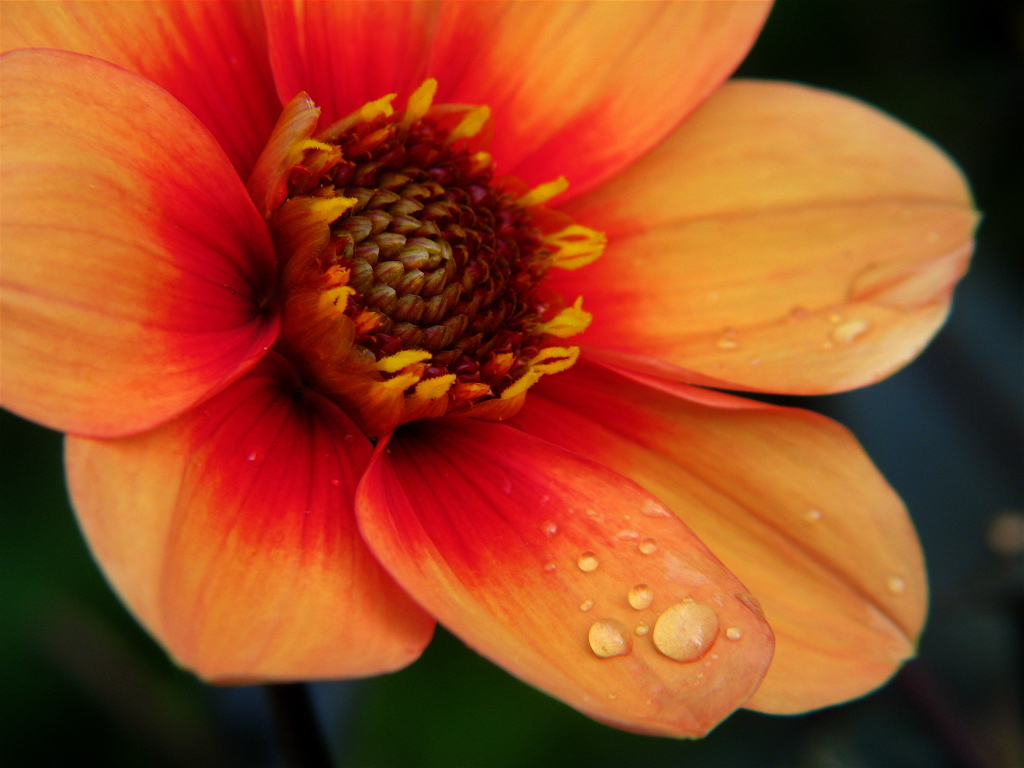
\includegraphics[scale=0.3]{figures/flower.jpg}
	\caption[Background segmentation]{
		The human visual system has no issue interpreting the subtle changes in translucency and shading in this photograph and segmenting the object from its background.
	}
	\label{flower}
\end{figure}

\section{Computer Vision}

As humans, we perceive the tridimensional structure of the world around us with apparent ease. Think of how vivid the tridimensional perception is when one looks at a vase of flowers sitting on the table. You can tell the shape and translucency of each petal through the subtle patterns of light and shading that play across its surface. One can easily segment
each flower from the background of the scene (see \autoref{flower}).

Looking at a framed group portrait, you can effortlessly for example count all of the people and even guess their emotions from their facial appearance. Perceptual psychologists have spent decades trying to understand how the visual system works and, even though they can find optical illusions to tease apart some of its principles (see \autoref{optical_illusion}), a solution to the complete puzzle remains elusive.

\begin{figure}[h]
	\centering
	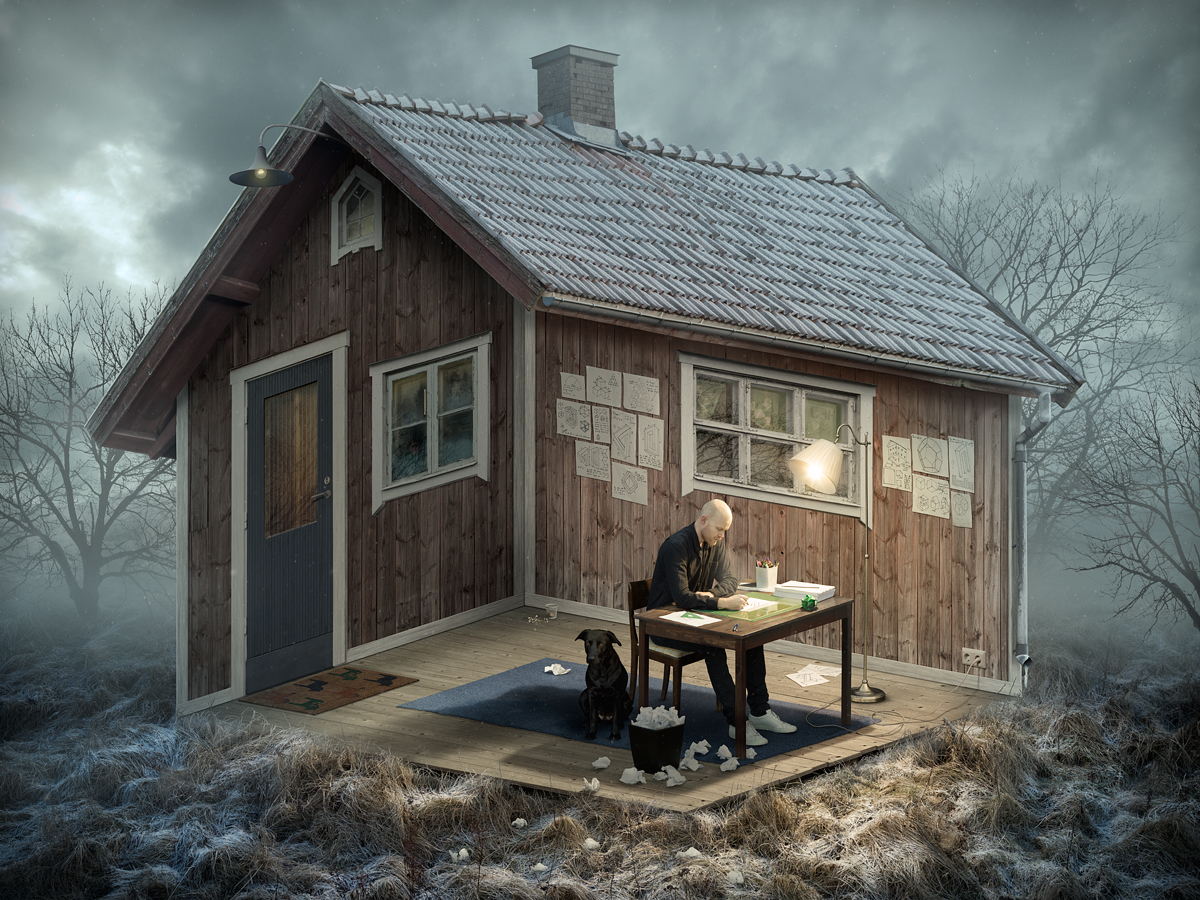
\includegraphics[scale=0.3]{figures/optical_illusion.jpg}
	\caption[Optical illusion]{
		 This work by Eric Johansson is composed of optical illusions that use highly creative pieces that render manipulations of perspective to make the viewer see a perplexed set of images. 
	}
	\label{optical_illusion}
\end{figure}

In areas, such as rendering a still scene composed of everyday objects or animating extinct creatures such as dinosaurs, the illusion of reality is almost perfect. In computer vision, we are trying to do the opposite, i.e., to describe the world that we see in one or a sequence of images and to reconstruct its properties, such as shape, illumination, and color distributions. It is incredible that humans and animals do this so effortlessly, while computer vision algorithms are so error prone.

Applications range from tasks such as industrial machine vision systems which, say, inspect bottles speeding by on a production line, to research into artificial intelligence and computers or robots that can comprehend the world around them. In many computer vision applications, the computers are preprogrammed to solve a certain task, but methods based on learning are now becoming more common. Examples of applications of computer vision include systems for:

\begin{itemize}
\item Process control.
\item Navigation.
\item Event detection. 
\item Information organization.
\item Object or environment modeling.
\item Interaction.
\item Automatic inspection.
\item Etc.
\end{itemize}

Each of the application areas described above employ a range of computer vision tasks; more or less well-defined measurement problems or processing workloads, which can be solved using a variety of methods. Some examples of typical computer vision tasks are presented below:

\begin{itemize}
\item \textbf{Recognition:} the classical problem in computer vision, image processing, and machine vision is that of determining whether or not the image data contains some specific object, feature, or activity.
\item \textbf{Motion analysis:} several tasks relate to motion estimation where an image sequence is processed to produce an estimate of the velocity either at each points in the image or in the 3D scene, or even of the camera that produces the images.
\item \textbf{Scene reconstruction:} Given one or (typically) more images of a scene, or a video, scene reconstruction aims at computing a 3D model of the scene.
\item \textbf{Image restoration:} The aim of image restoration is the removal of noise (sensor noise, motion blur, etc.) from images.
\end{itemize}

\begin{figure}
  \centering
  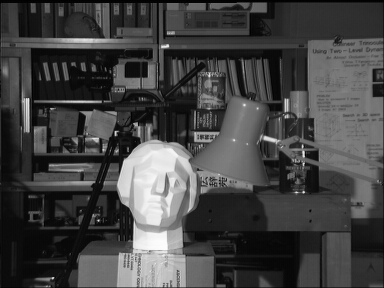
\includegraphics[width=0.475\textwidth]{figures/tsukuba_l.png} \quad
  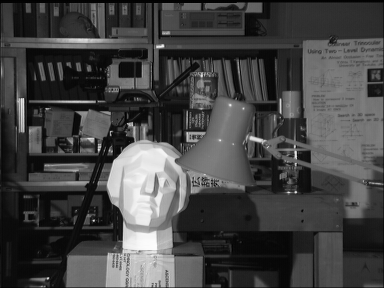
\includegraphics[width=0.475\textwidth]{figures/tsukuba_r.png}
  \caption{Example of stereoscopic images employed in scene reconstruction.}\label{tsukuba_ims}
\end{figure}

Our main interest in this project is \emph{scene reconstruction} from one or more pairs of images (see \autoref{tsukuba_ims}), specifically with stills obtained using stereo vision techniques. This images can be processed to obtain a depth estimation of the scene, once it is known, we have a 3D model of said scene.  

\subsection{Stereo Vision}

Any technique that is capable of collecting 3D information and creating the illusion of depth in an image, is considered stereoscopic vision or tridimensional (3D) vision. Our vision is stereoscopic by nature, being able to perceive the sensation of depth, distance, etc. This is achieved thanks to the horizontal separation between our eyes, leading to the processing of the differences between the perceived images of the visual system by our brain. 

Computer stereo vision is the extraction of 3D information from digital images, such as obtained by a CCD camera. Artificial systems for stereoscopic vision for the obtaining of 3D information in multiple applications, have been employed for several decades. The main problem that these systems tackle; is the determination of the correspondence between the pixels that come from the same point in the image pairs of the tridimensional scene. By comparing information about a scene from two vantage points, 3D data can be extracted by examination of the relative positions of objects in the two panels (see \autoref{stereo_vision}). %Wiki: https://en.wikipedia.org/wiki/Computer_stereo_vision

\begin{figure}[h]
	\centering
	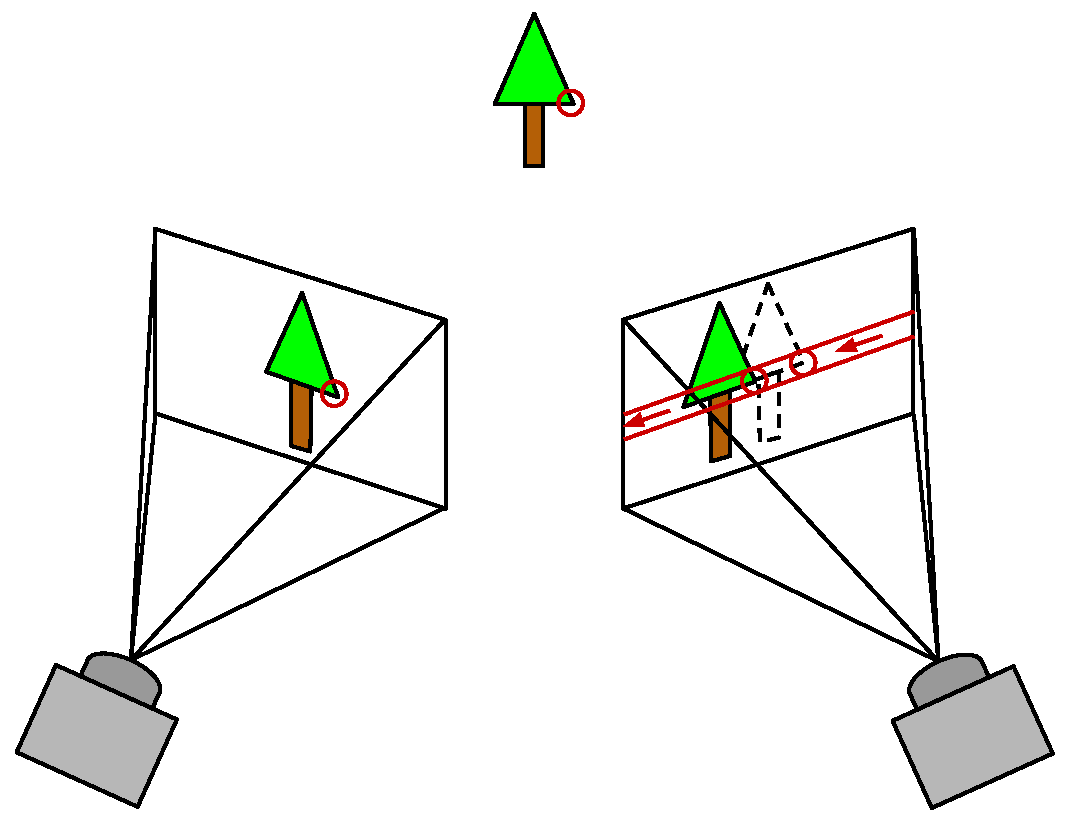
\includegraphics[scale=0.3]{figures/stereo_vision.pdf}
	\caption[Stereo vision]{
		 Diagram describing relationship of image displacement to depth with stereoscopic images, assuming flat co-planar images. 
	}
	\label{stereo_vision}
\end{figure}

\subsection{Stereo Correspondence}

Given two or more images of the same 3D scene, taken from different vantage points, the correspondence problem refers to the task of finding a set of points in one image which can be identified as the same points in another image. To achieve this, points or features in one image are matched with the corresponding points or features in another image. The images can be taken from a different point of view, not at the same time, or with objects in general motion relative to the cameras.

From the earliest forays into visual perception, it was known that we depth is perceived based on the differences in appearance between the left and right eye. As a simple test, hold your finger vertically in front of your eyes and close each eye at a time. You will notice that the finger jumps left and right, relative to the background of the image. The same effect is visible in the image pair shown in \autoref{tsukuba_depth}, in which the foreground objects shift left and right with respect to the background.

Stereo Matching is the process of employing two or more images and estimating a 3D model of the scene by finding matching areas of interest in the images and converting their 2D positions into 3D depths. This tackles the question of how to build a better 3D model, e.g., a sparse or dense depth map that assigns relative depths to pixels in the input images (see \autoref{tsukuba_depth}).

\begin{figure}[h]
  \centering
  \subfigure[Tsukuba left]{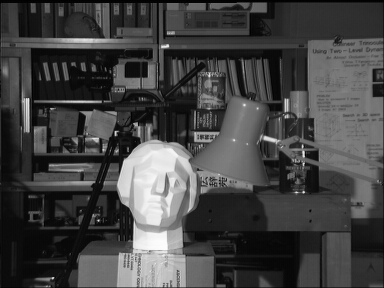
\includegraphics[width=0.29\textwidth]{figures/tsukuba_l.png}} \hfill
  \subfigure[Tsukuba right]{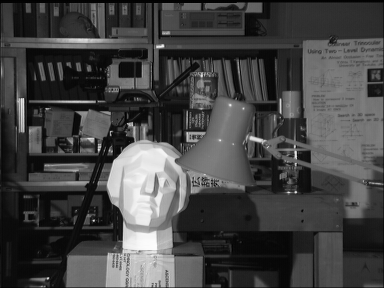
\includegraphics[width=0.29\textwidth]{figures/tsukuba_r.png}}\hfill
  \subfigure[Depth map]{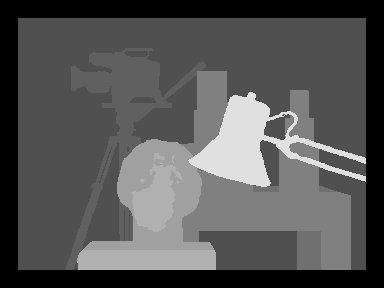
\includegraphics[width=0.29\textwidth]{figures/tsukuba_o_d.jpg}}
  \caption[Stereo reconstruction]{Stereo reconstruction techniques can convert (\textbf{a}-\textbf{b}) a pair of images, into (\textbf{c}) a depth map.}
  \label{tsukuba_depth}
\end{figure}

There are two main types of techniques for stereo matching:

\begin{itemize}
\item \textbf{Sparse} algorithms
\item \textbf{Dense} algorithms
\end{itemize}

Early stereo matching techniques were feature-based, i.e., they first extracted a set of potentially matchable image locations, using either interest operators or edge detectors, and then searched for matching locations in other images using a patch-based metric \cite{bolles1993jisct,hsieh1992performance}. This limitations to sparse correspondences were in part due to computational resource limitations, but also were driven by a need to limit the answers produced by algorithms to matches with high confidence.

While sparse matching algorithms are still used on occasion, most stereo matching algorithms today focus on dense correspondence. This came to be since it is required for applications, such as image-based rendering or modeling. This problem is more difficult than sparse correspondence, since inferring depth values in regions with similar textures requires making a certain amount of inferences.

After carefully studying multiple algorithms to achieve our goal, we have chosen Block Matching. This is not one of the algorithms with the highest precision, but we believe it can be highly parallel and fits our requirement of real-time processing of video images.

\begin{algorithm}[h]
	\DontPrintSemicolon
	\caption{Block Matching algorithm}
	\label{BMalgorithm}
	\KwIn{$left$, $right$, $aggregationdim$, $maxdisparity$}
	\KwOut{$depthmap$}
	\BlankLine
	$radius \leftarrow aggregationdim/2$\;
	\For{$x\leftarrow 0$ \KwTo $width$}{
		\For{$y\leftarrow 0$ \KwTo $height$}{
			$offsetx \leftarrow x - radius$\;
			$offsety \leftarrow y - radius$\;
			$sum \leftarrow 0$\;
			$bestsum \leftarrow -1$\;
			\For{$d\leftarrow 0$ \KwTo $maxdisparity$}{
				\For{$i\leftarrow offsetx$ \KwTo $aggregationdim + offsetx$}{	
					\For{$j\leftarrow offsety$ \KwTo $aggregationdim + offsety$}{
						$sum \leftarrow sum + \left | left[i * width + j] - left[i * width + j - d] \right |$\;
					}
				}
				\If{$sum < bestsum$}{
					$bestsum \leftarrow sum$\;
					$bestd \leftarrow d$\;
				}
				$sum \leftarrow 0$\;			
			}
			$depthmap[y * width + x] \leftarrow bestd$\;
		}
	}
\end{algorithm}

\subsection{Block Matching}

The chosen algorithm follows a similar structure to the following publication \cite{scharstein2002taxonomy}. With stereo cameras, objects in the field of view of these will appear at slightly different locations within the two images due to the cameras varying perspectives of the same scene. A standard method for calculating the disparity map is to use Block Matching, essentially, we will be taking a small region of pixels in the right image, and searching for the closest matching region of pixels in the left image. The structure and pseudo code of the implemented algorithm can be seen in \autoref{BMalgorithm}.

Correlation based matching typically produces dense depth maps by calculating the disparity at each pixel within a neighborhood. This is achieved by taking a square window of certain size around the pixel of interest in the reference image and finding the homologous pixel within the window in the target image, while moving along the corresponding scanline. The goal is to find the corresponding (correlated) pixel within a certain disparity range $d$ that minimizes the associated error and maximizes the similarity (see \autoref{window_search}).

%TODO source?
\begin{figure}[h]
	\centering
	\subfigure[Left image]{
\includegraphics[scale=0.4]{figures/left_wsearch_crop.png}}
	\subfigure[Right image search]{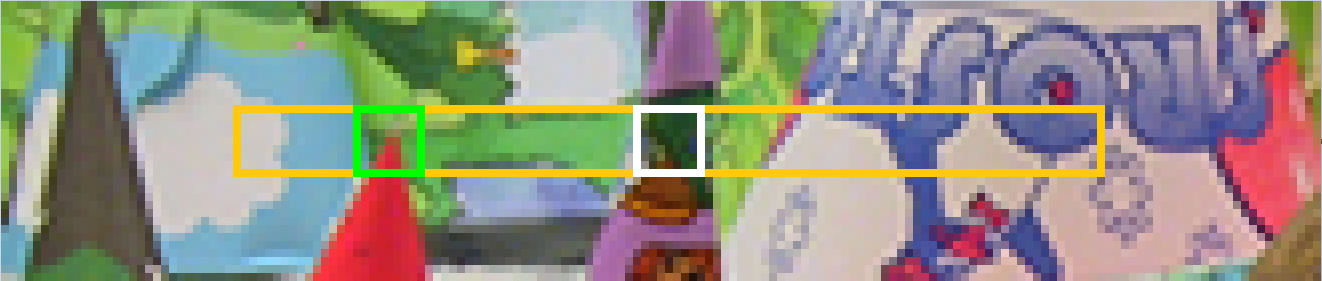
\includegraphics[scale=0.4]{figures/right_wsearch_crop.png}}
	\caption[Stereo vision]{
		 Diagram describing relationship of image displacement to depth with stereoscopic images, assuming flat co-planar images. 
	}
	\label{window_search}
\end{figure}

The most relevant part in this algorithm, is the comparison of the pixel windows between the left and right images. In our implementation we have implemented two approaches. The first, uses the following equation to calculate the \textit{Sum of Absolute Differences} (SAD) between pixels:

\begin{equation}\sum_{i,j\in W} \left | I_{l}(i,j) - I_{r}(i,j) \right |\end{equation}

Being $W$ the aggregation window dimension, $I_{l}$ the left image and $I_{r}$ the right image. The second uses a \textit{Sum of Squared Differences} (SSD) to achieve the same objective as we can observe in the next equation:

\begin{equation}\sum_{i,j\in W}  (I_{l}(i,j) - I_{r}(i,j))^2\end{equation}

Being $W$ the search window dimension, $I_{l}$ the left image and $I_{r}$ the right image. One of these calculations is repeated for pixel windows in the right image at a distance $d\in[0,disparity_{max}]$.

In short, the correspondence process involves the computation of the similarity measure for each disparity value, followed by an aggregation and optimization step. Since these steps consume a lot of processing power but can be computed in parallel, there are significant speed-performance advantages to be had in optimizing the matching algorithm.

\section{GPGPU}

\textit{General-purpose computing on graphics processing units} or GPGPU, is the use of a graphics processing unit (GPU), which typically handles computation only for computer graphics workloads, to perform calculations in applications traditionally handled by the central processing unit (CPU) \cite{fung2002mediated}. One can parallelize tasks even further using multiple graphics cards in one computer, or large numbers of graphics chips \cite{fung2004using}.

\subsection{Architecture}

Essentially, a GPGPU pipeline swaps data between one or more GPUs and CPUs and analyzes it as if it were in image or other graphic form. Because video cards can operate on 3D geometry and graphical data at speeds way faster than a traditional CPU, migrating data into graphical form and then using the GPU to process it and analyze it, can result in profound speed gains.

In a traditional \textbf{CPU architecture}, the CPU is able to access a large, general-purpose memory bank, called Random Access Memory (RAM) as is visually seen in \autoref{cpu_arch}.

\begin{figure}[h]
	\centering
	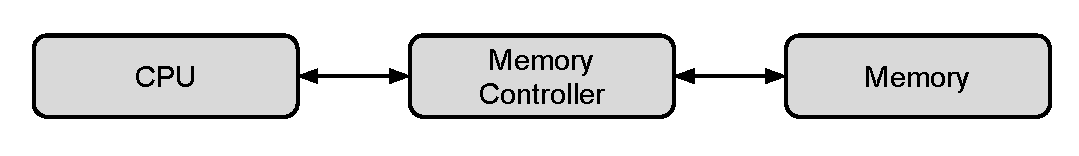
\includegraphics[scale=0.7]{figures/cpu_arch.pdf}
	\caption[CPU Architecture]{
	 Diagram describing a simplified CPU architecture. 
	}
	\label{cpu_arch}
\end{figure}

Nowadays, the CPU often contains more than one core, making CPUs capable of more than one task at a time.  This makes modern CPUs much faster than their single core, scalar predecessors.

In contrast, a \textbf{GPGPU architecture} uses \textit{Shared-Memory Multiprocessors} (SMP), these are a are a set of processors that all have their own local memory. These memory banks are shared within a thread group, but not between more than one of these groups.  However, each compute unit also has access to a global memory bank, which is shared between all processors.

\begin{figure}[h]
	\centering
	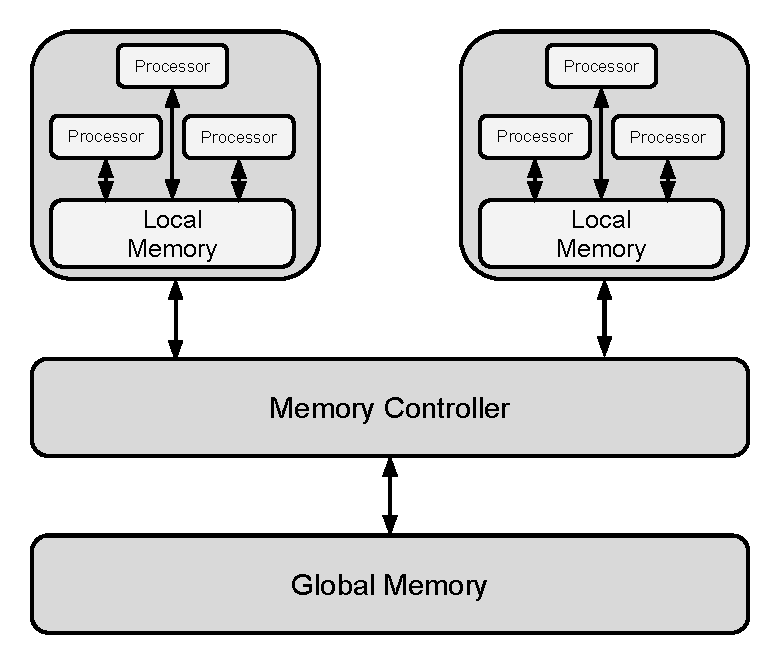
\includegraphics[scale=0.6]{figures/gpu_arch.pdf}
	\caption[GPU Architecture]{
	 Diagram showing a simplified SMP architecture. 
	}
	\label{gpu_arch}
\end{figure}

This is the parallel architecture that NVIDIA and AMD both use in their GPUs. Likewise, it is also the model enforced in the OpenCL and CUDA specification.

\subsection{OpenCL}

\textit{Open Computing Language} (OpenCL) is a framework for writing programs that make use of heterogeneous platforms consisting of CPUs, GPUs, digital signal processors (DSPs), field-programmable gate arrays (FPGAs) and other processors. OpenCL provides parallel computing using task-based and data-based parallelism. In addition, it is also an open standard maintained by the non-profit technology consortium Khronos Group \footnote{https://www.khronos.org/}.

OpenCL interprets a computing system as a number of heterogeneous compute devices, which might be CPUs or accelerators such as graphics processing units, attached to a host processor (a CPU). It defines a C-like language for writing programs, called kernels, that are later executed on the compute devices. A single compute device typically consists of several compute units, which in turn comprise multiple \textit{processing elements} (PEs). 

A single kernel execution may run on all or many of the PEs in parallel. How a compute device is subdivided into compute units and PEs depends on vendor criteria; a compute unit can be thought of as a CPU core, but the notion of core is hard to define across all the types of devices supported by OpenCL and the number of compute units may not correspond to the number of cores that the vendor can advertise.

\begin{figure}[h]
	\centering
	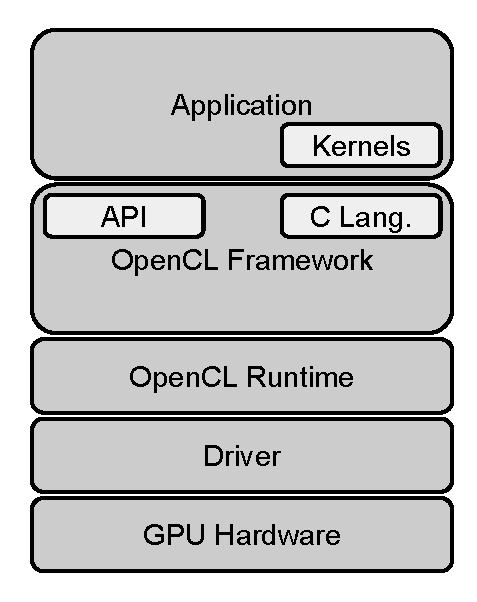
\includegraphics[scale=0.7]{figures/opencl_arch.pdf}
	\caption[OpenCL Architecture]{
	 Diagram showing the simplified OpenCL architecture. 
	}
	\label{opencl_arch}
\end{figure}

In addition to its this kernel programming language, OpenCL defines an \textit{application programming interface} (API) that allows normal programs running on the host to launch kernels on the compute devices and manage device memory, which is (at least conceptually) separate from host memory. Programs in the OpenCL language are intended to be compiled at run-time, so that applications that use OpenCL are portable between implementations for various host devices (see \autoref{opencl_arch}).

OpenCL defines a four-level memory hierarchy for the compute device:

\begin{itemize}
\item \textbf{Global memory:} Shared by all processing elements, but has high access latency.
\item \textbf{Read-only memory:} Smaller, low latency, writable by the host CPU but not the compute devices.
\item \textbf{Local memory:} Shared by a group of processing elements.
\item \textbf{Private memory:} Per-element private memory (registers).
\end{itemize}

\subsection{CUDA}

\textit{Compute Unified Device Architecture} (CUDA) is a parallel computing platform and application programming interface (API) model created by NVIDIA. It allows software developers to use CUDA-enabled GPUs for general purpose processing. The CUDA platform is a software layer that gives direct access to the virtual instruction set and parallel computational elements of GPUs.

In contrast with OpenCL, this is a proprietary framework and is not compatible with such a varied array of devices, CUDA is only compatible with NVIDIA GPUs. It is compatible with programming languages such as C, \CC and Fortran. This makes it easier for specialists in parallel programming to utilize GPU resources, as opposed to previous API solutions like Direct3D and OpenGL, which required advanced skills in graphics programming.

\begin{figure}[h]
	\centering
	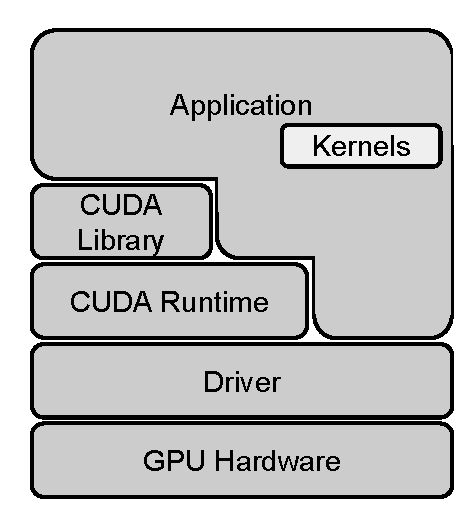
\includegraphics[scale=0.7]{figures/cuda_arch.pdf}
	\caption[CUDA Architecture]{
	 Diagram showing the simplified CUDA architecture. 
	}
	\label{CUDA_arch}
\end{figure}

Another difference between OpenCL and CUDA is how applications are compiled. In OpenCL kernels are compiled ad-hoc with the OpenCL framework, while in CUDA we will use a custom copiler called NVCC to compile the complete application or the parts that contain CUDA code. The CUDA architecture is built around a scalable array of multiprocessors, each one of them having several scalar processors, one multi-threading unit, and a shared memory chip. The multiprocessors are able to create, manage, and execute parallel threads, with a small overhead. The threads are grouped in blocks, which are executed in a single multiprocessor, and the blocks are grouped into grids. When a CUDA program calls a grid to be executed in the GPU, each one of the blocks in the grid is numbered and distributed to an available multiprocessor. When a multiprocessor receives a block to execute, it splits the threads in warps, a set of 32 consecutive threads. Each warp executes a single instruction at a time, so the best efficiency is achieved when the 32 threads in the warp executes the same instruction. Each time that a block finishes its execution, a new block is assigned to the available multiprocessor. 

CUDA defines a similar memory hierarchy for compute devices:

\begin{itemize}
\item \textbf{Global memory:} Shared by all processing elements, but has high access latency.
\item \textbf{Read-only memory:} Smaller, low latency, writable by the host CPU but not the compute devices.
\item \textbf{Shared memory:} Shared by a block of threads.
\item \textbf{Local memory:} Per-thread local memory.
\item \textbf{Register memory:} Per-thread registers.
\end{itemize}
	%
% T�TULO DEL CAP�TULO
%
\chapter{GCVL: GPU Computer Vision Library
	\label{chapter_3}
}

\textbf{GCVL} is a set of software tools and libraries that allow the user to run and implement common Computer Vision algorithms on modern GPUs. It comprises a set of OpenCL and CUDA tools, a Block Matching example algorithm implementation and base classes to implement custom algorithms.

\section{Development Methodology}

Agile software development \cite{agiledev} is a combination of development methods that use iterative and incremental development, where requirements and solutions mature through collaboration between self-organizing, cross-functional teams. The motto of this method is ``embrace change''; that is why it encourages adaptive planning, evolutionary development and delivery, a time-boxed iterative approach, and promotes quick and flexible response to change.

\subsection{Agile manifesto}

In February of 2001, several developers met at Snowbird, Utah resort, to debate different lightweight development methods. They published the \emph{Manifesto for Agile Software Development} \cite{agilemani} to define the approach that is now called agile software development. 

The conclusions that we can reach from the manifesto's items are described below:

\begin{itemize}
\item \textbf{Individuals and Interactions}: In agile development self-organization and motivation are really important. Other values promoted by the manifesto are co-location\footnote{The act of placing multiple individuals within a single location.} and pair programming\footnote{Two programmers work together at one workstation.}.
\item \textbf{Working software}: Working software will be utilized for more purposes than presenting documents to the client.
\item \textbf{Customer collaboration}: The software requirements cannot be fully realized from the beginning of the software development cycle, so being in touch with the customer is really important.
\item \textbf{Responding to change}: Agile development is keen on fast responses to change and continuous development.  
\end{itemize}

More principles are mentioned in the manifesto, some of them are:

\begin{itemize}
\item Customer satisfaction by rapid delivery of useful software.
\item Welcome changes even late in the development.
\item Working software is the principal measure of progress.
\item Maintaining a constant pace.
\item Cooperation between business people and developers. 
\item Build projects around motivated individuals.
\item Attention to technical excellence.
\item Simplicity.
\end{itemize}

Agile methods break down tasks into small increments with minimal planning and normally long-term planning is not directly involved. \emph{Iterations} are short timeframes that typically last from one to four weeks. A team works in each iteration through a full software development cycle; including planning, requirements analysis, design, coding, etc. This minimizes risk and facilitates adaptation to change. An iteration may not add enough new functionalities to warrant a market release, but the objective is to have an available release at the end of each iteration. 

Team composition does not depend on corporate hierarchies or corporate roles of team members. They normally have the responsability of completing tasks that deliver the required functionalities that an iteration requires. How to meet an iteration's objectives is decided individually.

The ``weight'' of the method depends on the type of project, the planning and order of tasks in a generalist project should not be the same as in a research project.  

Agile methods encourage face-to-face communication instead of written documents if possible. Most teams work in an open office (the \emph{bullpen}), which makes this type of communication easier. 

Each agile team contains a customer representative, that ensures that customer needs and company goals are aligned. 

Most agile methods encourage a routine that includes daily face-to-face communication among team members. In a brief session team members tell each other what they achieved the previous day, what they are going to do today and the problems that have appeared. 

As agile development emphasizes on working software as the primary measure of progress and has a clear preference in face-to-face communication this results in less written documentation than other methods. This does not mean that documentation should be disregarded, but that less emphasis is made on documentation because is not needed as much.

\section{Design}

GCVL is developed following an object oriented approach and using the \CC programming language. For GPGPU programming we have chosen OpenCL and CUDA, because of their inter-operation capabilities with OpenGL. This will allow us to process directly data that already resides in the GPU, without having to do expensive memory transfers. Because of the open nature of OpenCL, the software will be able to run on any graphics card vendor (AMD, NVIDIA or Intel) and the SO that the user prefers (Windows, OSX or Unix). For NVIDIA GPUs we have also developed a CUDA implementation, this way users will be able to squish the maximum amount of performance out of the green team's devices. Design patterns have been used as much as possible. This section briefly depicts the high-level design of GCVL in the form of class diagrams.

\subsection{Class diagram}

The high-level design of the \textbf{GCVL} library is depicted in the class diagram of \autoref{class_diag}. In this design, the \textbf{General Tools} module contains utility classes that contain commonly used functions and configuration parameters. In addition, the \textbf{CPU} module contains tools to implement multi-core CPU algorithms using GCVL, examples, template classes, etc.

\begin{figure}[h]
	\centering
	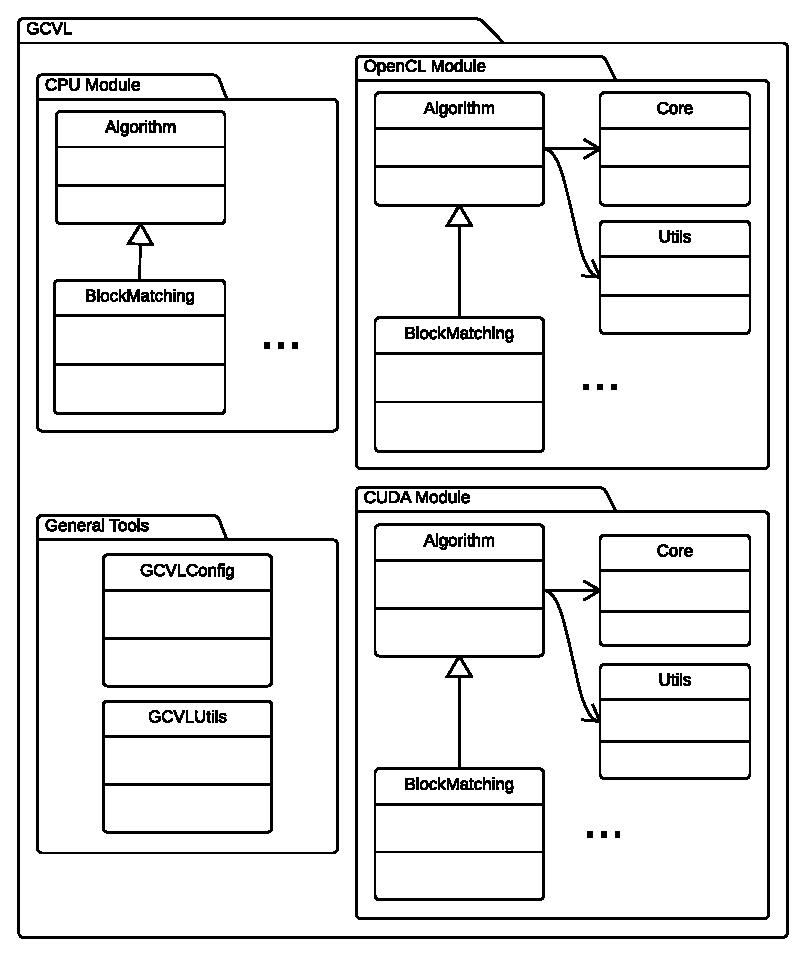
\includegraphics[scale=0.73]{figures/GCVL.pdf}
	\caption{GCVL class diagram.} \label{class_diag}
\end{figure}

Furthermore, the \textbf{OpenCL} module contains classes related to the development of OpenCL algorithms (tools, example algorithms, kernels, etc.).

Finally, the \textbf{CUDA} module resembles the aforementioned module, containing tools, algorithm examples, kernels, etc. It possesses all the classes that are needed to implement CUDA programs in a simple manner.

All of the GPU modules present in GCVL can be compiled on demand using CMake options, so if the CUDA framework or the OpenCL libraries are not needed, they can be deactivated and the rest of the library can be used without any kind of issue.

\subsection{General Tools}

\begin{figure}[h]
	\centering
	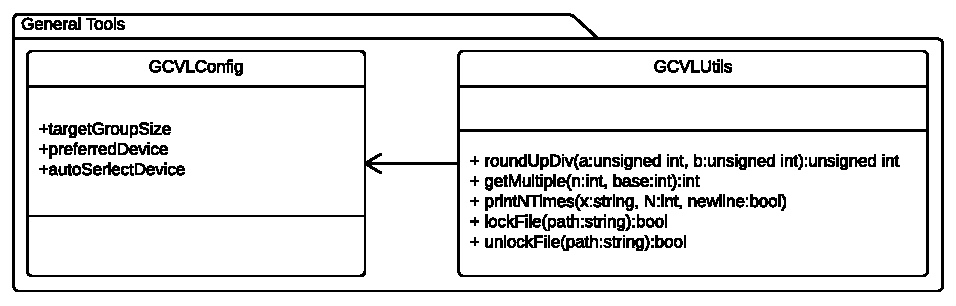
\includegraphics[scale=0.73]{figures/general_tools.pdf}
	\caption{General Tools module class diagram.} \label{general_tools}
\end{figure} 

In the diagram of \autoref{general_tools}, the following classes are the most relevant:

\begin{itemize}
	\item \textbf{GCVLConfig:} This class contains the configuration parameters present in GCVL. For example, the suppression of warnings, constant definitions, etc. 
	\item \textbf{GCVLTools:} Class that contains utility functions used in all the modules present in GCVL, be it CPU or GPU modules. 
\end{itemize}

\subsection{CPU Module}

This is a GPGPU oriented computation library, but it also provides code for multi-core CPUs. The
relevant classes are shown in the class diagram \autoref{cpu_module}:

\begin{itemize}
	\item \textbf{Algorithm:} This base class contains the template for the implementation  of multi-core CPU algorithms in GCVL.
	\item \textbf{BlockMatching:} This class serves as an example of the implementation of a multi-core CPU algorithm in GCVL. 
\end{itemize}

\begin{figure}[h]
	\centering
	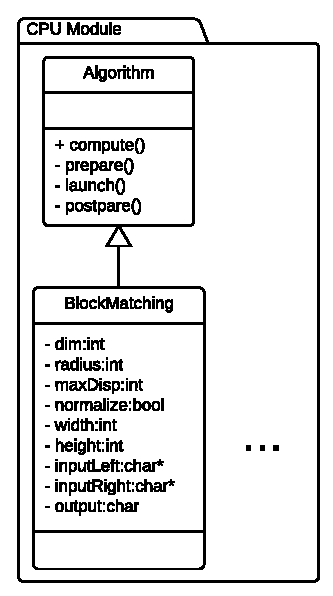
\includegraphics[scale=0.73]{figures/cpu_module.pdf}
	\caption{CPU module class diagram.} \label{cpu_module}
\end{figure} 

\subsection{OpenCL Module}

\begin{figure}[h]
	\centering
	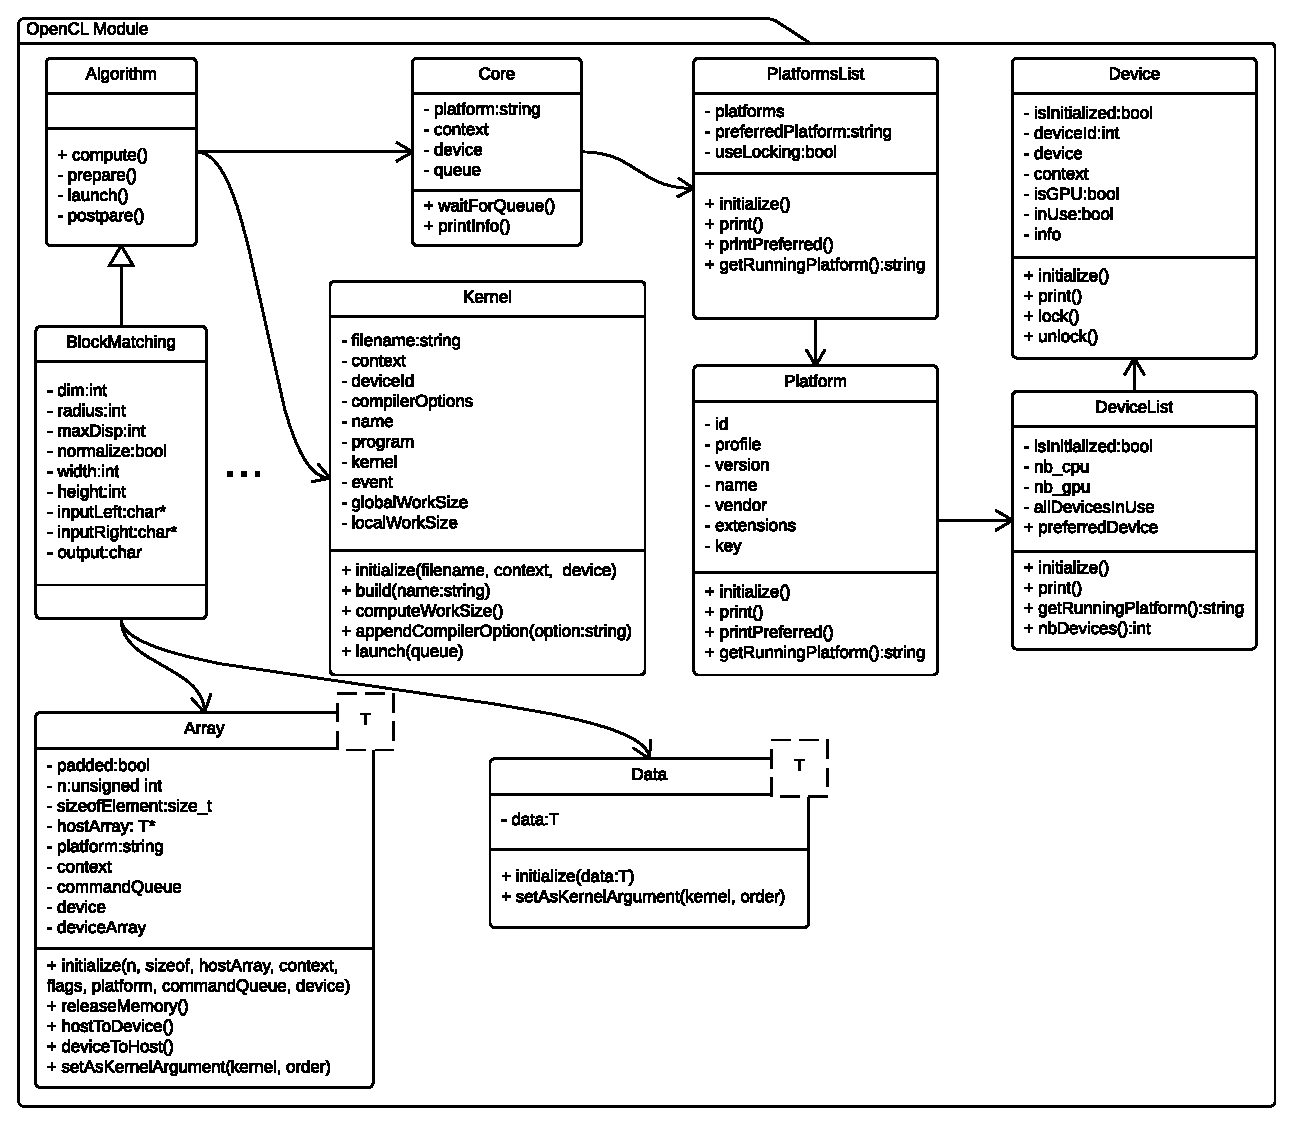
\includegraphics[scale=0.73]{figures/opencl_module.pdf}
	\caption{OpenCL module class diagram.} \label{opencl_module}
\end{figure} 

Since this is a GPU computing library, the first related module is the OpenCL module. In it, classes, algorithms, kernels that belong to the OpenCL implementation are packed together for convenience in the \textbf{opencl} name space. The most significant classes related to the management of the OpenCL algorithms are shown in the class diagram of \autoref{opencl_module}:

\begin{itemize}
	\item \textbf{Algorithm:} This base class contains the template for the implementation  of OpenCL algorithms in GCVL.
	\item \textbf{BlockMatching:} This class serves as an example of the implementation of a OpenCL algorithm in GCVL.
	\item \textbf{Core:} Class in charge of the creation of OpenCL platforms, selection of the best GPU, creation of queues, etc.  
	\item \textbf{Platform:} Helper class that aids in the creation of a certain computing platform. AMD, NVIDIA, Intel, etc.
	\item \textbf{PlatformsList:} Class that holds a list with all the available platforms in the system.
	\item \textbf{Device:} Utility class that aids in the creation of compute devices.
	\item \textbf{DevicesList:} Class that holds a list of all the compute devices available in a platform and tries to guess the best one.
	\item \textbf{Kernel:} Wrapper class for the creation of kernels in OpenCL.
	\item \textbf{Array:} Helper class for OpenCL device array creation.
	\item \textbf{Data:} Utility class for the creation of OpenCL device data.
\end{itemize}

\subsection{CUDA Module}

\begin{figure}[h]
	\centering
	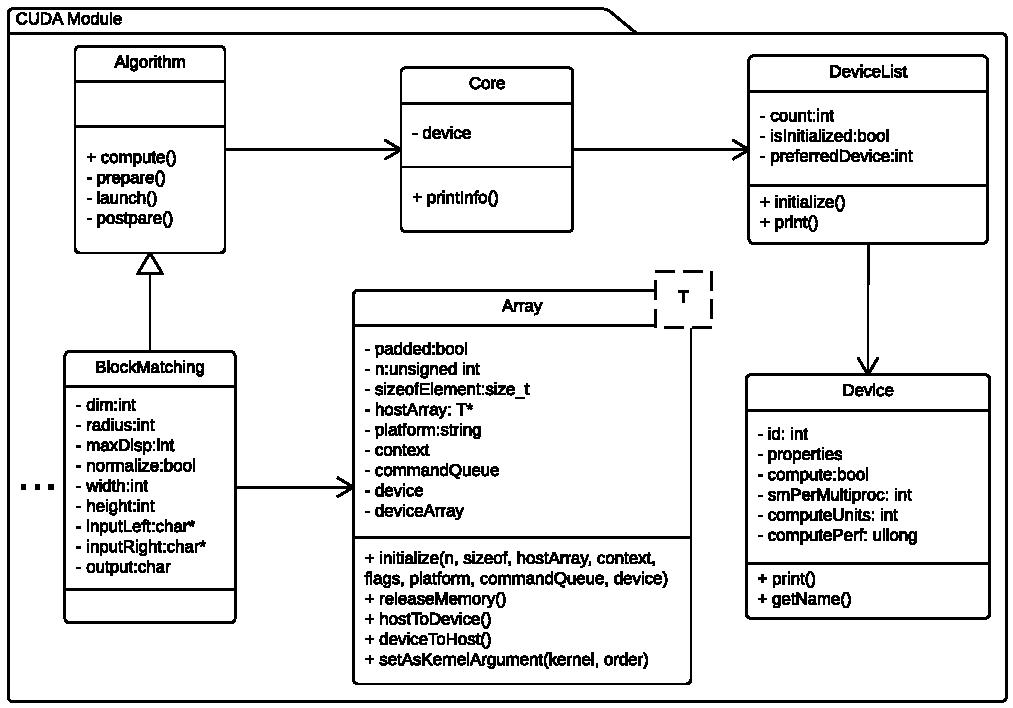
\includegraphics[scale=0.73]{figures/cuda_module.pdf}
	\caption{CUDA module class diagram.} \label{cuda_module}
\end{figure} 

The second GPU computing module gives the user the choice of using CUDA to implement GPU related algorithms using the \textbf{cuda} name space. The most relevant classes explained here are present in the class diagram in \autoref{cuda_module}:

\begin{itemize}
	\item \textbf{Algorithm:} This base class contains the template for the implementation  of CUDA algorithms in GCVL.
	\item \textbf{BlockMatching:} This class serves as an example of the implementation of a CUDA algorithm in GCVL. 
	\item \textbf{Core:} Class in charge of the creation of the CUDA environment, selection of the best GPU, creation device arrays, etc. 
	\item \textbf{Device:} Utility class that aids in the instantiation of compute devices.
	\item \textbf{DevicesList:} Class that holds a list of all the compute devices available in the system. In addition, it tries to guess the best one depending on architecture, compute units and clock speed.
	\item \textbf{Array:} Helper class for CUDA device array creation.
\end{itemize}

\section{Technology}

%TODO complete
Tecnologia usada?

\section{Usage}

Once the design concepts behind GCVL have been explained, the only task left is to know how the modules are used. We will first see how to run the CPU module algorithms, next we will see how the OpenCL module works and last but not least we will see how the CUDA module can be utilized to run the CUDA algorithms.

\subsection{CPU Module}

The CPU module usage is pretty straightforward, one only needs to include the corresponding algorithm class; in our example it will be the BlockMatching algorithm (see \autoref{cpu_bm_example}). In this example, the two paths of the input images and the output image pointer are passed to the BlockMatching class, next the BlockMatching settings are set and the computation is started. The result will be available to the user in the output pointer.

\lstset{language=C++,frame=shadowbox,rulesepcolor=\color[gray]{0.8},lineskip=10pt, 
		keywordstyle=\color{VioletRed}\bfseries,
		emph={Core,BlockMatching}, emphstyle=\color{Emerald}\bfseries, basicstyle=\footnotesize,
		emph={[2]setAggDim,setMaxDisp,setNormalize,compute}, emphstyle={[2]\color{PineGreen}}}
\begin{lstlisting}[float,caption={How to use the BlockMatching class.},captionpos=b,label={cpu_bm_example}]
	#include <gcvl/blockmatching.h>
	int main(int argc, char *argv[]) {
		int dim = 5, maxDisp = 16;
		bool norm = true;
		std::unique_ptr<unsigned char[]> output; 
		gcvl::BlockMatching bm(argv[1], argv[2], output);
		bm.setAggDim(dim);
		bm.setMaxDisp(maxDisp);
		bm.setNormalize(norm);
		bm.compute();
	}
\end{lstlisting}

\subsection{OpenCL Module}

The OpenCL module inner workings are a little more complex, but its usage is still really simple. The first step is to include the corresponding algorithm class and Core class; in our example it will be the BlockMatching algorithm (see \autoref{ocl_bm_example}). In this case, the core, the two paths of the input images and the output image pointer are passed to the BlockMatching class. Next, the BlockMatching settings are set and the computation is started. The result will be available to the user in the output pointer.

\begin{lstlisting}[float,caption={How to use the OpenCL BlockMatching class.},captionpos=b,label={ocl_bm_example}]
	#include <gcvl/opencl/oclcore.h>
	#include <gcvl/opencl/oclblockmatching.h>
	int main(int argc, char *argv[]) {
		int dim = 5, maxDisp = 16;
		bool norm = true;
		std::unique_ptr<unsigned char[]> output;	 
		gcvl::opencl::Core core;
		gcvl::opencl::BlockMatching bm(core, argv[1], argv[2], output);
		bm.setAggDim(dim);
		bm.setMaxDisp(maxDisp);
		bm.setNormalize(norm);
		bm.compute();
	}
\end{lstlisting}

\subsection{CUDA Module}

The CUDA module is used in a similar manner to the OpenCL module, but using a different namespace. The first step is to include the corresponding algorithm class and Core class; in our example it will be the BlockMatching algorithm (see \autoref{cuda_bm_example}). In this case, the core, the two paths of the input images and the output image pointer are passed to the BlockMatching class. Next, the BlockMatching settings are set and the computation is started. The result will be available to the user in the output pointer.

\begin{lstlisting}[float,caption={How to use the CUDA BlockMatching class.},captionpos=b,label={cuda_bm_example}]
	#include <gcvl/cuda/cudacore.h>
	#include <gcvl/cuda/cudablockmatching.h>
	int main(int argc, char *argv[]) {
		int dim = 5, maxDisp = 16;
		bool norm = true;
		std::unique_ptr<unsigned char[]> output;	 
		gcvl::cuda::Core core;
		gcvl::cuda::BlockMatching bm(core, argv[1], argv[2], output);
		bm.setAggDim(dim);
		bm.setMaxDisp(maxDisp);
		bm.setNormalize(norm);
		bm.compute();
	}
\end{lstlisting}

	%
% T�TULO DEL CAP�TULO
%
\chapter{Performance \& Experimental Results
	\label{chapter_4}
}

intro

\section{Performance Results}

performance

\section{Experimental Results}

experiments
	%
% T�TULO DEL CAP�TULO
%
\chapter{Conclusions and future lines of work
	\label{chapter_5}
}

In this chapter we will briefly take a look at the conclusions reached after finishing this project, and the possible future lines of work that the project can follow.

\section[Conclusions]{Conclusions}

The first conclusion reached, has been that all of the objectives of the project were met:

\begin{itemize}
\item Studying different Stereo Matching techniques.
\item Design, implementation and documentation of tools to ease GPGPU programming.
\item Design, implementation and documentation of the chosen algorithm. 
\item CPU parallelization of the implemented algorithm.
\item GPU parallelization of the implemented algorithm.
\end{itemize}

After finishing and achieving the aforementioned objectives, the other conclusions that have been reached are:

\begin{itemize}
\item \textbf{GPGPU is not always the answer:} As seen in the results, if the workload is not complex enough to compensate for kernel setup time, GPU computation time will be higher than the time it takes the CPU to process the data. One has to carefully consider if the workload and the chosen algorithms are optimal for GPU parallelization or a lot of time can be wasted.
\end{itemize} 

\section[Future lines of work]{Future lines of work}

After finalizing the work on this project, several ideas for the expansion of the visualizer come to mind:

\begin{itemize}
\item \textbf{GPU kernels optimization:} As of know the implemented kernels of the Block Matching algorithm are semi-naive implementations. It would be interesting to further optimize these kernels so they would use local memory and would access the data with more optimal patterns or other types of improvements.
\item \textbf{Multi-GPU:}
\item \textbf{MPI tools:}
\item \textbf{Boost Compute:}
\end{itemize} 

	% INCLUIMOS LOS AP�NDICES...
        %\appendix
	%\include{tfg_appendix_010}
%         \include{tfg_appendix_020}

	%Primero hay que compilar el bibtex para que salga.
	% INCLUIMOS LA BIBLIOGRAF�A...
	\nocite{*}	% Se usa para indicar en la bibliograf�a las referencias no citadas.
	\bibliography{pfm_biblio}
	\bibliographystyle{alpha}

\end{document}

